\documentclass[tikz,border=10pt]{standalone}
\begin{document}
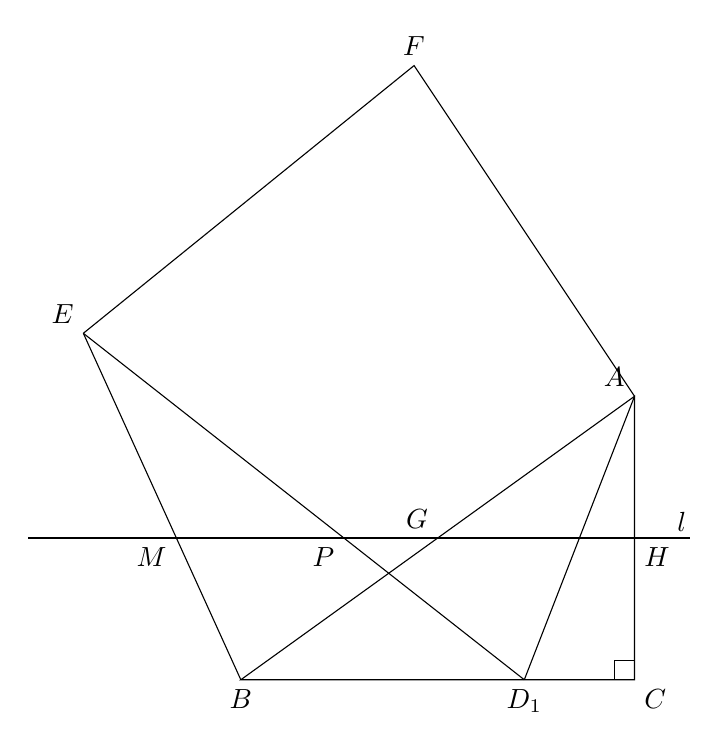
\begin{tikzpicture}[scale=1]
  \coordinate (A) at (7,3.6);
  \coordinate (B) at (2,0);
  \coordinate (C) at (7,0);
  \coordinate (D1) at (5.6,0);
  \coordinate (E) at (0,4.4);
  \coordinate (F) at (4.2,7.8);
  \coordinate (M) at (1.18,1.8);
  \coordinate (P) at (3.31,1.8);
  \coordinate (G) at (4.5,1.8);
  \coordinate (H) at (7,1.8);

  % triangle / square edges
  \draw (A) -- (B) -- (C) -- cycle;
  \draw (A) -- (D1);
  \draw (B) -- (D1);
  \draw (E) -- (B);
  \draw (E) -- (D1);
  \draw (E) -- (F) -- (A);

  % line l
  \draw (-0.7,1.8) -- (7.7,1.8);

  % right-angle mark at C
  \draw (6.75,0) -- (6.75,0.25) -- (7,0.25);

  % labels
  \node[above left] at (A) {$A$};
  \node[below] at (B) {$B$};
  \node[below right] at (C) {$C$};
  \node[below] at (D1) {$D_1$};
  \node[above left] at (E) {$E$};
  \node[above] at (F) {$F$};
  \node[below left] at (M) {$M$};
  \node[below left] at (P) {$P$};
  \node[above left] at (G) {$G$};
  \node[below right] at (H) {$H$};
  \node at (7.6,2.0) {$l$};
\end{tikzpicture}
\end{document}
